%\externaldocument{appendix_tor_model}
\chapter{Appendix for Structural Changes in Doped and Excited Conjugated Polymers}\label{append:tor_model}

\section{Polythiophene Torsion Potentials}
\label{sec:pt_tp}
\subsection{Torsion Potential Data and Initial Structures}
\begin{table}[hbt!]\centering
\caption{Ground-state Thiophene Dimer Initial Structure}
\renewcommand{\arraystretch}{1.5}
\begin{threeparttable}
\begin{tabular}{ccccc}\toprule
{} & {Atom} & {X (\AA)} & {Y (\AA)} & {Z (\AA)} \\ \midrule
  1 & S & -0.0023723 & -0.0560977 & -0.0300969\\
  2 & C & 1.7070035 & -0.0292241 & -0.0145267\\
  3 & H & 2.2421009 & -0.0503556 & 0.9188681\\
  4 & C & 2.2188238 & 0.0166957 & -1.2731976\\ \midrule
  5 & H & 3.2760435 & 0.0396095 & -1.4857363\\
  6 & C & 1.2080458 & 0.0437755 & -2.2700460\\
  7 & H & 1.4022626 & 0.1035054 & -3.3303301\\
  8 & C & -0.0534481 & 0.0159971 & -1.7485209\\ \midrule
  9 & C & -1.3283732 & 0.0357503 & -2.4552048\\
  10 & C & -2.5140867 & 0.5793303 & -2.0518483\\
  11 & H & -2.6304470 & 1.0993723 & -1.1131149\\
  12 & C & -3.5508397 & 0.4152358 & -3.0079307\\ \midrule
  13 & H & -4.5565336 & 0.7819288 & -2.8760054\\
  14 & C & -3.1332923 & -0.2472315 & -4.1192789\\
  15 & H & -3.7048930 & -0.4997928 & -4.9952883\\
  16 & S & -1.4859744 & -0.6908589 & -4.0068121\\ \bottomrule
\end{tabular}
\begin{tablenotes}
\item
\end{tablenotes}
\end{threeparttable}
\end{table}

\begin{table}[hbt!]\centering
\caption{Ground-state Thiophene Dimer Torsion Data}
\renewcommand{\arraystretch}{1.5}
\begin{threeparttable}
\begin{tabular}{cccc}\toprule
  {} & {Torsion Angle} & {Rel. Energy (eV)} & {Abs. Energy (Hartree)} \\ \midrule
    1 & 0.0 & 0.04598 & -1104.84987203842\\
    2 & 10.0 & 0.03979 & -1104.85009939477\\
    3 & 20.0 & 0.02779 & -1104.85054035879\\
    4 & 30.0 & 0.01928 & -1104.85085335093\\ \midrule
    5 & 40.0 & 0.01868 & -1104.85087543253\\
    6 & 50.0 & 0.02689 & -1104.85057349252\\
    7 & 60.0 & 0.04200  & -1104.85001836446\\
    8 & 70.0 & 0.05898 & -1104.84939439490\\ \midrule
    9 & 80.0 & 0.07241 & -1104.84890093182\\
    10 & 90.0 & 0.07646 & -1104.84875201328\\
    11 & 100.0 & 0.06924 & -1104.84901713984\\
    12 & 110.0 & 0.05278 & -1104.84962222807\\ \midrule
    13 & 120.0 & 0.03288 & -1104.85035334414\\
    14 & 130.0 & 0.01530 & -1104.85099955470\\
    15 & 140.0 & 0.00358 & -1104.85143006908\\
    16 & 150.0 & 0.00000 & -1104.85156180070\\ \midrule
    17 & 160.0 & 0.00326 & -1104.85144196165\\
    18 & 170.0 & 0.00927 & -1104.85122115615\\
    19 & 180.0 & 0.01234 & -1104.85110839823\\ \bottomrule
\end{tabular}
\begin{tablenotes}
\item
\end{tablenotes}
\end{threeparttable}
\end{table}

\begin{table}[hbt!]\centering
\caption{Doped-state Thiophene Dimer Initial Structure}
\renewcommand{\arraystretch}{1.5}
\begin{threeparttable}
\begin{tabular}{ccccc}\toprule
{} & {Atom} & {X (\AA)} & {Y (\AA)} & {Z (\AA)} \\ \midrule
  1 & S & 0.0003979 & 0.4373270 & -0.0633642\\
  2 & C & 1.6743230 & 0.2163099 & -0.0571461\\
  3 & H & 2.2287328 & 0.3339913 & 0.8611866\\
  4 & C & 2.1929799 & -0.1115590 & -1.3041171\\ \midrule
  5 & H & 3.2426659 & -0.2866798 & -1.4795321\\
  6 & C & 1.2098407 & -0.1839581 & -2.2716885\\
  7 & H & 1.3925319 & -0.4251174 & -3.3088107\\
  8 & C & -0.0772964 & 0.0912069 & -1.7653271\\ \midrule
  9 & C & -1.2859459 & 0.1035335 & -2.4670641\\
  10 & C & -2.5730754 & 0.3787571 & -1.9607149\\
  11 & H & -2.7557610 & 0.6199609 & -0.9236020\\
  12 & C & -3.5562300 & 0.3062435 & -2.9282622\\ \midrule
  13 & H & -4.6059215 & 0.4813222 & -2.7528378\\
  14 & C & -3.0375815 & -0.0216838 & -4.1752213\\
  15 & H & -3.5920046 & -0.1394621 & -5.0935336\\
  16 & S & -1.3636358 & -0.2425520 & -4.1690348\\ \bottomrule
\end{tabular}
\begin{tablenotes}
\item
\end{tablenotes}
\end{threeparttable}
\end{table}

\begin{table}[hbt!]\centering
\caption{Doped-state Thiophene Dimer Torsion Data}
\renewcommand{\arraystretch}{1.5}
\begin{threeparttable}
\begin{tabular}{cccc}\toprule
  {} & {Torsion Angle} & {Rel. Energy (eV)} & {Abs. Energy (Hartree)} \\ \midrule
    1 & 0.0 & 0.02079 & -1104.50938633204\\
    2 & 10.0 & 0.02825 & -1104.50911231215\\
    3 & 20.0 & 0.05223 & -1104.50823104848\\
    4 & 30.0 & 0.09371 & -1104.50670665615\\ \midrule
    5 & 40.0 & 0.15812 & -1104.50433961960\\
    6 & 50.0 & 0.24644 & -1104.50109374877\\
    7 & 60.0 & 0.35673 & -1104.49704060708\\
    8 & 70.0 & 0.48820 & -1104.49220922909\\ \midrule
    9 & 80.0 & 0.63920 & -1104.48666033352\\
    10 & 90.0 & 0.78498 & -1104.48130300611\\
    11 & 100.0 & 0.62139 & -1104.48731456600\\
    12 & 110.0 & 0.47554 & -1104.49267465589\\ \midrule
    13 & 120.0 & 0.34797 & -1104.49736261553\\
    14 & 130.0 & 0.24010 & -1104.50132673110\\
    15 & 140.0 & 0.15423 & -1104.50448240244\\
    16 & 150.0 & 0.08729 & -1104.50694235511\\ \midrule
    17 & 160.0 & 0.03966 & -1104.50869281167\\
    18 & 170.0 & 0.01087 & -1104.50975071487\\
    19 & 180.0 & 0.00000 & -1104.51015031856\\ \bottomrule
\end{tabular}
\begin{tablenotes}
\item
\end{tablenotes}
\end{threeparttable}
\end{table}

\begin{table}[hbt!]\centering
\caption{Excited-state Thiophene Dimer Initial Structure}
\renewcommand{\arraystretch}{1.5}
\begin{threeparttable}
\begin{tabular}{ccccc}\toprule
{} & {Atom} & {X (\AA)} & {Y (\AA)} & {Z (\AA)} \\ \midrule
  1 & S & -0.0180675 & 0.4466192 & -0.0408593\\
  2 & C & 1.6926804 & 0.2166109 & -0.0439241\\
  3 & H & 2.2550459 & 0.3305548 & 0.8671136\\
  4 & C & 2.1935848 & -0.1115653 & -1.3030670\\ \midrule
  5 & H & 3.2449313 & -0.2870510 & -1.4774923\\
  6 & C & 1.2341910 & -0.1883271 & -2.2796908\\
  7 & H & 1.4178092 & -0.4288461 & -3.3154027\\
  8 & C & -0.1008011 & 0.0925904 & -1.7763147\\ \midrule
  9 & C & -1.2624454 & 0.1021336 & -2.4560715\\
  10 & C & -2.5974302 & 0.3830769 & -1.9527024\\
  11 & H & -2.7810468 & 0.6236319 & -0.9169985\\
  12 & C & -3.5568312 & 0.3062823 & -2.9293227\\ \midrule
  13 & H & -4.6081778 & 0.4817637 & -2.7548939\\
  14 & C & -3.0559380 & -0.0219757 & -4.1884438\\
  15 & H & -3.6183064 & -0.1359654 & -5.0994740\\
  16 & S & -1.3451782 & -0.2518931 & -4.1915259\\ \bottomrule
\end{tabular}
\begin{tablenotes}
\item
\end{tablenotes}
\end{threeparttable}
\end{table}

\begin{table}[hbt!]\centering
\caption{Excited-state Thiophene Dimer Torsion Data}
\renewcommand{\arraystretch}{1.5}
\begin{threeparttable}
\begin{tabular}{cccc}\toprule
  {} & {Torsion Angle} & {Rel. Energy (eV)} & {Abs. Energy (Hartree)} \\ \midrule
    1 & 0.0 & 0.01269 & -1104.69509558720\\
    2 & 10.0 & 0.02498 & -1104.69464387418\\
    3 & 20.0 & 0.06486 & -1104.69317837941\\
    4 & 30.0 & 0.13225 & -1104.69070196155\\ \midrule
    5 & 40.0 & 0.22992 & -1104.68711247641\\
    6 & 50.0 & 0.36069 & -1104.68230686926\\
    7 & 60.0 & 0.50986 & -1104.67682512101\\
    8 & 70.0 & 0.64448 & -1104.67187782963\\ \midrule
    9 & 80.0 & 0.75853 & -1104.66768637840\\
    10 & 90.0 & 0.84183 &  -1104.66462531896\\
    11 & 100.0 & 0.76183 & -1104.66756522231\\
    12 & 110.0 & 0.65961 & -1104.67132193500\\ \midrule
    13 & 120.0 & 0.53077 & -1104.67605665532\\
    14 & 130.0 & 0.38036 & -1104.68158410041\\
    15 & 140.0 & 0.24551 & -1104.68653968278\\
    16 & 150.0 & 0.13895 & -1104.69045559904\\ \midrule
    17 & 160.0 & 0.06376 & -1104.69321900264\\
    18 & 170.0 & 0.01692 & -1104.69494025977\\
    19 & 180.0 & 0.00000 & -1104.69556201328\\ \bottomrule
\end{tabular}
\begin{tablenotes}
\item
\end{tablenotes}
\end{threeparttable}
\end{table}

\clearpage
\subsection{Ground-state Torsion Potentials at Different Levels of Theory}
\
\begin{figure}[hbt!]
    \centering
    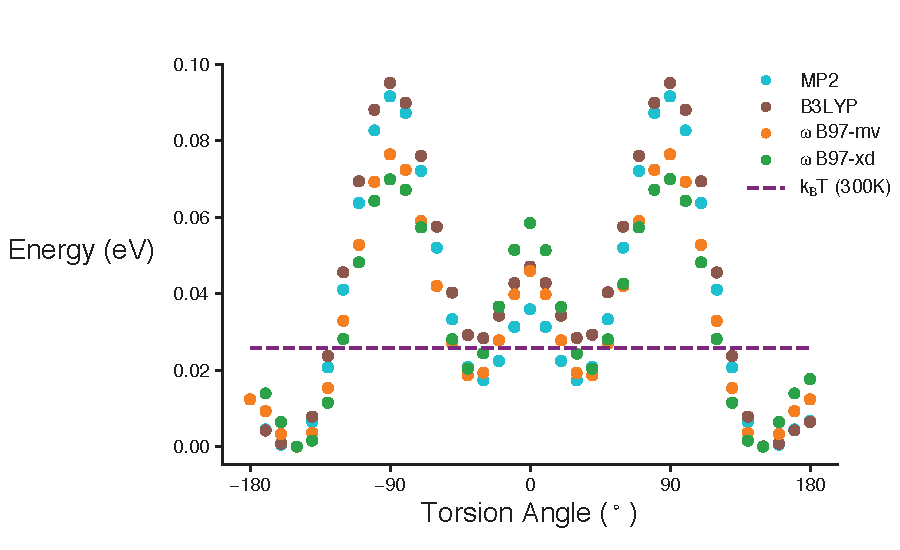
\includegraphics{figures/append_tor_model/SI_compare_theory_torsion.pdf}
    \caption{Ground-state torsion potential at different levels of theory. MP2 basis set: cc-pVTZ, B3LYP and $\omega$B97-xd basis set: 6-31++G**, $\omega$B97-mv basis set: def2-QZVPPD}
    \label{fig:gs_theory}
\end{figure}

\subsection{The Effect of Chain Length on Ground-state Torsion Angles}
\label{subsec:chain_length_gs}

Different polythiophene (PT) chain lengths were optimized at the RI-MP2 level (Figure \ref{tab:gs_RIMP2}). In all instances the optimized structures had non-planar central torsion angles corresponding to minima observed in Figure \ref{fig:gs_theory}. Additionally, the energy of optimized planar (trans) configurations were higher than that of optimized non-planar configurations. This evidence supports DuBay et al. in their claim that the torsion potential of conjugated polymers such as PT can be approximated by the dimer torsion potential if an appropriate level of theory, basis set, and optimization procedure are used.\cite{Dubay2012}

\begin{table}[hbt!]\centering
\caption{Ground-state Optimized Geometries}
\label{tab:gs_RIMP2}
\renewcommand{\arraystretch}{1.5}
\begin{threeparttable}
\begin{tabular}{cccc}\toprule
\multicolumn{1}{c}{\multirow{2}{2.5cm}{\centering Number of \\ Monomers}} &
\multicolumn{1}{c}{\multirow{2}{4.1cm}{\centering Trans Geometry \\ Abs. Energy (Hartree)}} &
\multicolumn{1}{c}{\multirow{2}{4.1cm}{\centering Optimized Geometry \\ Abs. Energy (Hartree)}} &
\multicolumn{1}{c}{\multirow{2}{4.1cm}{\centering Optimized Central  \\ Torsion Angle ($^\circ$)}} \\ \\ \midrule
    2 & -1103.35246329362\tnote{a} & -1103.35284395916\tnote{a} & 22\\
    4 & -2205.26456300358\tnote{b} & -2205.26519616574\tnote{b} & 161\\
    8 & -- & -4409.36496730408\tnote{b} & 159\\ \bottomrule
\end{tabular}
\begin{tablenotes}
\item[a] \footnotesize Theory: RI-MP2 basis set: cc-pVQZ
\item[b] \footnotesize Theroy: RI-MP2 basis set: cc-pVTZ
\end{tablenotes}
\end{threeparttable}
\end{table}

\clearpage

\subsection{The Effect of Chain Length on Doped Torsion Potentials}
\label{subsec:chain_length_cat}

The impact of chain length was investigated for doped torsion potentials to address concerns about charge and spin localization. In the end, the dimer approximation was suitable as it was in the ground state. The relaxation procedure detailed in the main text was altered for doped chains longer than $n = 4$ due to the polaron shifting away from the central torsion of interest for non-planar configurations. Shifting of the polaron can be seen in figures \ref{fig:n6_bl} and \ref{fig:n8_bl} where the bond length distortion moves from the center to one of edges, while the $N = 2$ and $N = 4$ chains were too short for the polaron to have anywhere to shift (Figure \ref{fig:n2_bl} and \ref{fig:n4_bl}). The modified relaxation procedure for the $N = 6$ and $N = 8$ doped chains consisted of an initial geometry optimization followed by single point energy calculations at each torsional configuration. This procedure maintained the position of the polaron on the central torsion angle of interest.

\begin{figure}[hbt!]
    \centering
    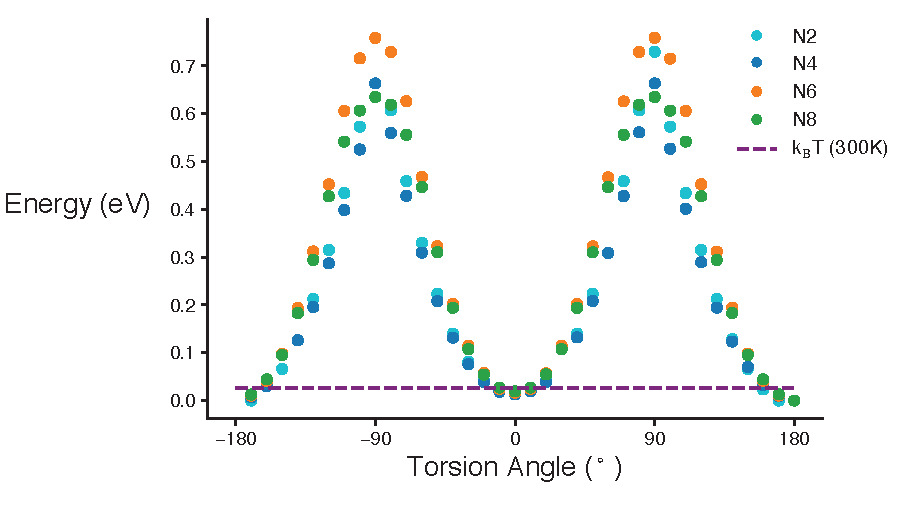
\includegraphics{figures/append_tor_model/SI_cat_diff_lens.pdf}
    \caption{Doped (cation) torsion potential for different chain lengths (N monomers). Functional: $\omega$B97-xd basis set: 6-31++G** }
    \label{fig:cat_dl}
\end{figure}

\begin{figure}[hbt!]
    \centering
    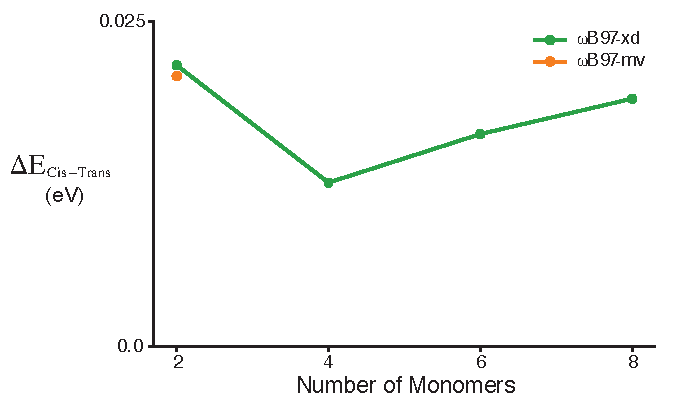
\includegraphics{figures/append_tor_model/delta_e_plot.pdf}
    \caption{The relative energy between trans and cis configurations at different chain lengths}
    \label{fig:delta_e}
\end{figure}

\clearpage
\begin{table}[hbt!]\centering
\captionsetup{justification=centering}
\captionsetup{width=.6\textwidth}
\captionsetup{skip=2pt}
\caption{Relative Energy Differences Between the Cis and the Trans Ground-state Configurations}
\renewcommand{\arraystretch}{1.5}
\begin{threeparttable}
\begin{tabular}{cccc}\toprule
  {Number of Monomers} & {$\Delta E_{ \ Cis - Trans}$ (eV)} \\ \midrule
    2 & 0.02079\tnote{a}\\
    2 & 0.02162\tnote{b}\\
    4 & 0.01260\tnote{b}\\
    6 & 0.01633\tnote{b}\\
    8 & 0.01905\tnote{b}\\ \bottomrule
\end{tabular}
\begin{tablenotes}
\item[a] \footnotesize Functional: $\omega$B97-mv basis set: def2-QZVPPD
\item[b] \footnotesize Functional: $\omega$B97-xd basis set: 6-31++G**
\end{tablenotes}
\end{threeparttable}
\end{table}

\begin{figure}[hbt!]
    \centering
    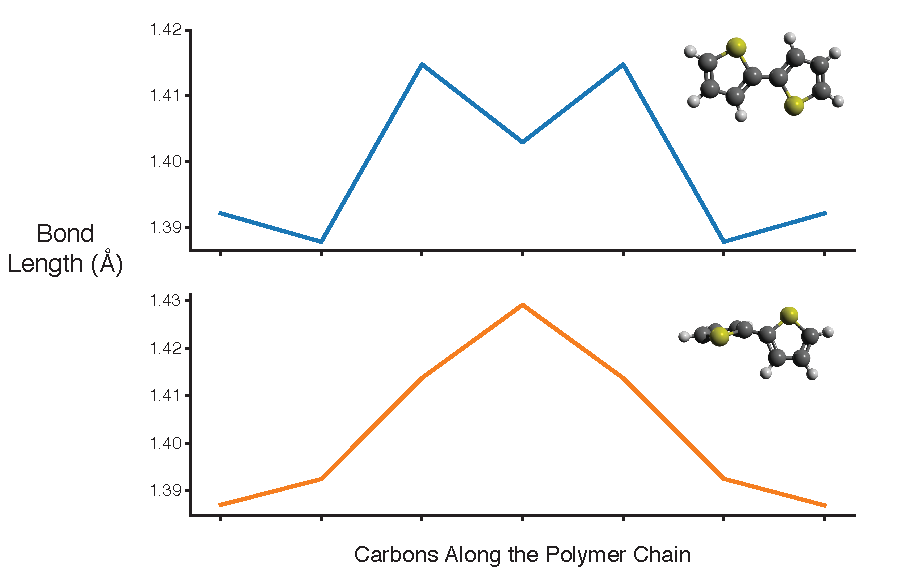
\includegraphics{figures/append_tor_model/n2_fig_w.pdf}
    \caption{Carbon-Carbon bond lengths along the doped (cation) dimer. Top: Relaxed planar configuration, Bottom: Relaxed twisted configuration}
    \label{fig:n2_bl}
\end{figure}

\begin{figure}[hbt!]
    \centering
    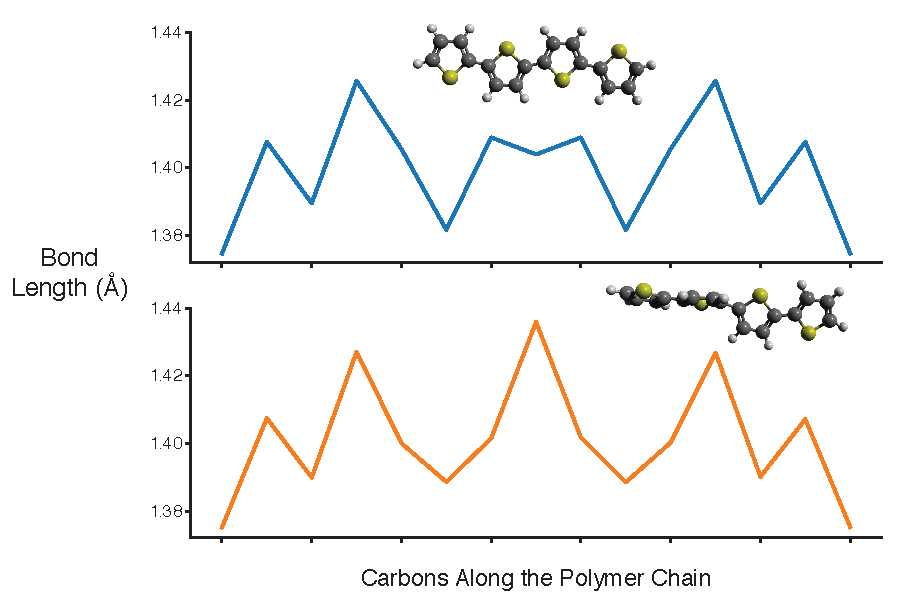
\includegraphics{figures/append_tor_model/n4_fig_w.pdf}
    \caption{Carbon-Carbon bond lengths along the doped (cation) $N = 4$ chain. Top: Relaxed planar configuration, Bottom: Relaxed twisted configuration}
    \label{fig:n4_bl}
\end{figure}

\begin{figure}[hbt!]
    \centering
    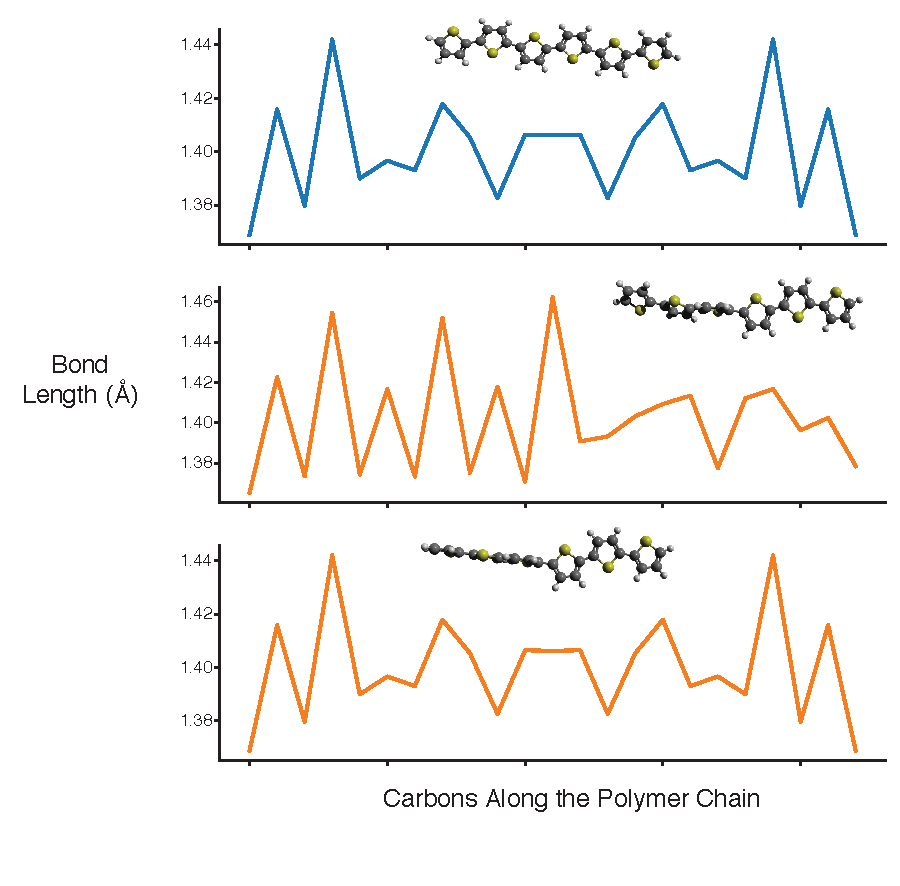
\includegraphics{figures/append_tor_model/n6_fig_w.pdf}
    \caption{Carbon-Carbon bond lengths along the doped (cation) $N = 6$ chain. Top: Relaxed planar configuration, Middle: Relaxed twisted configuration, Bottom: Frozen twisted configuration}
    \label{fig:n6_bl}
\end{figure}

\begin{figure}[hbt!]
    \centering
    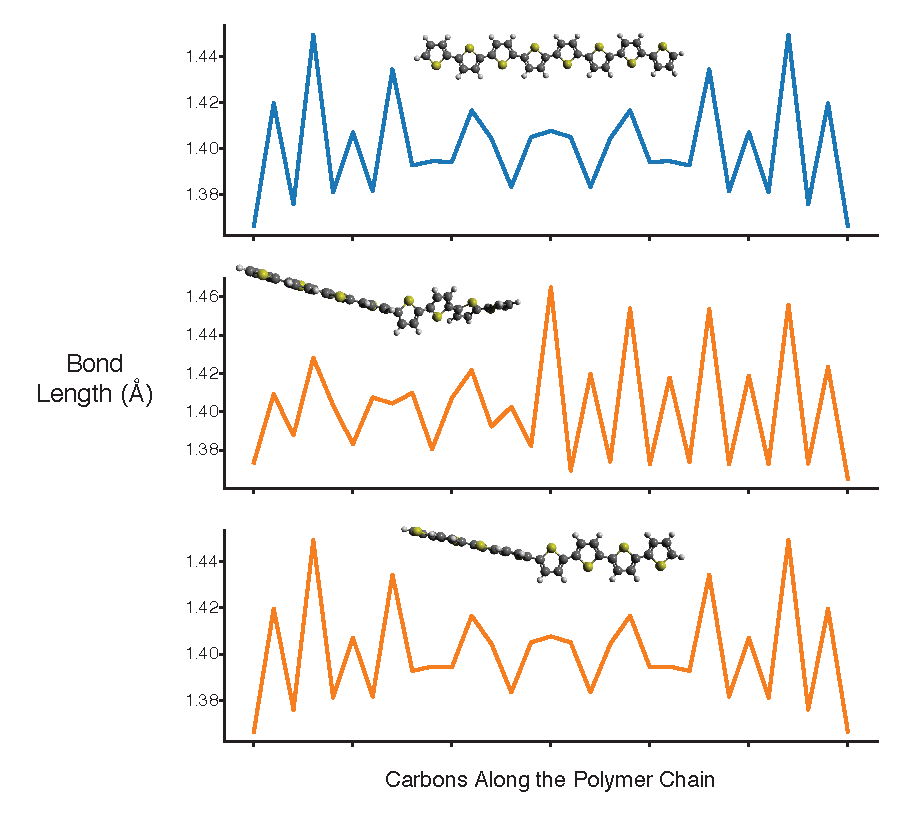
\includegraphics{figures/append_tor_model/n8_fig_w.pdf}
    \caption{Carbon-Carbon bond lengths along the doped (cation) $N = 8$ chain. Top: Relaxed planar configuration, Middle: Relaxed twisted configuration, Bottom: Frozen twisted configuration}
    \label{fig:n8_bl}
\end{figure}

\clearpage

\subsection{Excited Torsion Potentials at Different Levels of Theory}

Previous work on organic conjugated molecules demonstrated that RO-DFT and UO-DFT were better than TDDFT at reproducing experimental electronic properties for the first triplet state (T1).\cite{Hait2016} Nevertheless, TDDFT, RO-DFT, and UO-DFT were compared in table \ref{tab:ex_ct_gap} to understand the magnitude of energy differences between the theories.

\begin{table}[hbt!]\centering
\captionsetup{justification=centering}
\captionsetup{width=.6\textwidth}
\captionsetup{skip=2pt}
\caption{Relative Energy Differences Between the Cis and the Trans Excited (T1) Configurations}
\label{tab:ex_ct_gap}
\renewcommand{\arraystretch}{1.5}
\begin{threeparttable}
\begin{tabular}{cccc}\toprule
\multicolumn{1}{c}{\multirow{1}{3.5cm}{\centering }} &
\multicolumn{1}{c}{\multirow{1}{3.5cm}{\centering $\Delta E_{\ Cis - Trans}$ (eV)}} \\ \midrule
    TDDFT\tnote{\textdagger} & 0.02137\\
    UO-DFT\tnote{\textdagger} & 0.01338\\
    UO-DFT\tnote{*} & 0.01269\\
    RO-DFT\tnote{*} & 0.01609\\ \bottomrule
\end{tabular}
\begin{tablenotes}
\item[\textdagger] \footnotesize Functional: $\omega$B97-xd basis set: 6-31++G**
\item[*] \footnotesize Functional: $\omega$B97-mv basis set: def2-TZVPPD
\end{tablenotes}
\end{threeparttable}
\end{table}

\section{Polypyrrole Torsion Potentials}
\label{sec:ppy}
\subsection{Torsion Potential Comparison}

\begin{figure}[hbt!]
    \centering
    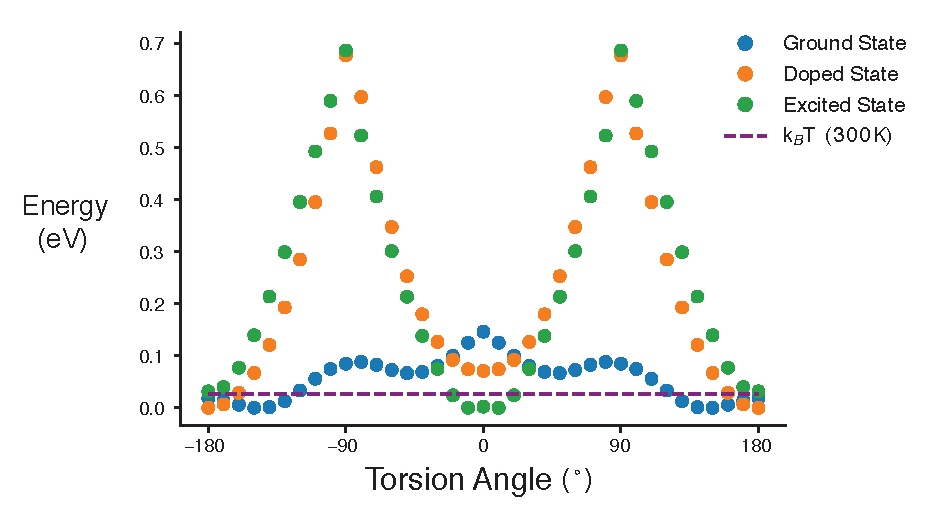
\includegraphics{figures/append_tor_model/ppy_torsion_compare.pdf}
    \caption{A comparison of the ground, doped (cation), and excited-state (first triplet) torsion potentials of pyrrole dimer molecules. Functional: $\omega$B97-mv basis set: def2-TZVPPD}
    \label{fig:ppy_tor}
\end{figure}

The pyrrole torsion potentials were assumed to symmetric (i.e. only calculating the positive half of the potential) as they were with thiophene (See Subsection \ref{sec:TPF}\ref{subsec:TPF_descript}). We note that all the excited-state configurations had out-of-plane N-H hydrogens, whereas the doped-state configurations had all in plane N-H hydrogens.

\clearpage

\subsection{Torsion Potential Data and Initial Structures}
\begin{table}[hbt!]\centering
\caption{Ground-state Pyrrole Dimer Initial Structure}
\renewcommand{\arraystretch}{1.5}
\begin{threeparttable}
\begin{tabular}{ccccc}\toprule
{} & {Atom} & {X (\AA)} & {Y (\AA)} & {Z (\AA)} \\ \midrule
    1  & N &  0.1438107 & -0.0411429 & -0.4535532\\
    2  & C &  1.4773229 & -0.0788175 & -0.1493554\\
    3  & H &  1.8151739 & -0.1383387 &  0.8700846\\
    4  & C &  2.1764672 & -0.0299186 & -1.3248901\\
    5  & H &  3.2487461 & -0.0316715 & -1.4199869\\
    6  & C &  1.2270605 &  0.0405707 & -2.3794193\\ \midrule
    7  & H &  1.4372125 &  0.1342226 & -3.4320510\\
    8  & C & -0.0250831 &  0.0289564 & -1.8102511\\
    9  & C & -1.3498064 &  0.0805442 & -2.4043013\\
    10 & C & -2.5284819 &  0.6262933 & -1.9518871\\
    11 & H & -2.6535219 &  1.1765257 & -1.0340344\\
    12 & C & -3.5191498 &  0.3838374 & -2.9409496\\ \midrule
    13 & H & -4.5519255 &  0.6856820 & -2.9082884\\
    14 & C & -2.9158139 & -0.2956872 & -3.9643888\\
    15 & H & -3.3097283 & -0.6661324 & -4.8941293\\
    16 & N & -1.6006395 & -0.4734122 & -3.6306845\\
    17 & H & -0.6104249 & -0.1240319 &  0.2028327\\
    18 & H & -0.9253188 & -0.9915794 & -4.1617169\\ \bottomrule
\end{tabular}
\begin{tablenotes}
\item
\end{tablenotes}
\end{threeparttable}
\end{table}

\begin{table}[hbt!]\centering
\caption{Ground-state Pyrrole Dimer Torsion Data}
\renewcommand{\arraystretch}{1.5}
\begin{threeparttable}
\begin{tabular}{cccc}\toprule
  {} & {Torsion Angle} & {Rel. Energy (eV)} & {Abs. Energy (Hartree)} \\ \midrule
    1  & 0.0   & 0.14631 & -419.150251034421\\
    2  & 10.0  & 0.12506 & -419.151031655173\\
    3  & 20.0  & 0.09972 & -419.151963159215\\
    4  & 30.0  & 0.08050 & -419.152669398895\\ \midrule
    5  & 40.0  & 0.06897 & -419.153092977519\\
    6  & 50.0  & 0.06674 & -419.153175077438\\
    7  & 60.0  & 0.07273 & -419.152954901242\\
    8  & 70.0  & 0.08265 & -419.152590252506\\ \midrule
    9  & 80.0  & 0.08828 & -419.152383572136\\
    10 & 90.0  & 0.08456 & -419.152520200073\\
    11 & 100.0 & 0.07462 & -419.152885388511\\
    12 & 110.0 & 0.05579 & -419.153577293422\\ \midrule
    13 & 120.0 & 0.03306 & -419.154412807997\\
    14 & 130.0 & 0.01279 & -419.155157674912\\
    15 & 140.0 & 0.00121 & -419.155583069180\\
    16 & 150.0 & 0.00000 & -419.155627663140\\ \midrule
    17 & 160.0 & 0.00582 & -419.155413621542\\
    18 & 170.0 & 0.01394 & -419.155115472566\\
    19 & 180.0 & 0.01848 & -419.154948650234\\ \bottomrule
\end{tabular}
\begin{tablenotes}
\item
\end{tablenotes}
\end{threeparttable}
\end{table}

\begin{table}[hbt!]\centering
\caption{Doped-state Pyrrole Dimer Initial Structure}
\renewcommand{\arraystretch}{1.5}
\begin{threeparttable}
\begin{tabular}{ccccc}\toprule
{} & {Atom} & {X (\AA)} & {Y (\AA)} & {Z (\AA)} \\ \midrule
    1  & N &  0.1244013 & -0.0124993 & -0.4386263\\
    2  & C &  1.4375902 & -0.0551168 & -0.1587828\\
    3  & H &  1.7929559 & -0.0891701 &  0.8573685\\
    4  & C &  2.1557384 & -0.0461157 & -1.3603672\\
    5  & H &  3.2278057 & -0.0736121 & -1.4461102\\
    6  & C &  1.2344603 &  0.0037460 & -2.3853068\\ \midrule
    7  & H &  1.4529189 &  0.0231124 & -3.4400252\\
    8  & C & -0.0592961 &  0.0253156 & -1.8067791\\
    9  & C & -1.3176295 &  0.0746973 & -2.4037290\\
    10 & C & -2.6113886 &  0.0961671 & -1.8252036\\
    11 & H & -2.8298491 &  0.0767245 & -0.7704869\\
    12 & C & -3.5326670 &  0.1460190 & -2.8501433\\ \midrule
    13 & H & -4.6047365 &  0.1734334 & -2.7644022\\
    14 & C & -2.8145161 &  0.1551214 & -4.0517254\\
    15 & H & -3.1698811 &  0.1892087 & -5.0678758\\
    16 & N & -1.5013265 &  0.1125333 & -3.7718813\\
    17 & H & -0.6094801 & -0.0090223 &  0.2491140\\
    18 & H & -0.7674401 &  0.1092375 & -4.4596173\\ \bottomrule
\end{tabular}
\begin{tablenotes}
\item
\end{tablenotes}
\end{threeparttable}
\end{table}

\begin{table}[hbt!]\centering
\caption{Doped-state Pyrrole Dimer Torsion Data}
\renewcommand{\arraystretch}{1.5}
\begin{threeparttable}
\begin{tabular}{cccc}\toprule
  {} & {Torsion Angle} & {Rel. Energy (eV)} & {Abs. Energy (Hartree)} \\ \midrule
    1  & 0.0   & 0.07089 & -418.901257453274\\
    2  & 10.0  & 0.07429 & -418.901132469421\\
    3  & 20.0  & 0.09209 & -418.900478404582\\
    4  & 30.0  & 0.12671 & -418.899206193558\\ \midrule
    5  & 40.0  & 0.17981 & -418.897254678549\\
    6  & 50.0  & 0.25308 & -418.894562034780\\
    7  & 60.0  & 0.34742 & -418.891095239250\\
    8  & 70.0  & 0.46244 & -418.886868205963\\ \midrule
    9  & 80.0  & 0.59734 & -418.881910697353\\
    10 & 90.0  & 0.67736 & -418.878970154026\\
    11 & 100.0 & 0.52725 & -418.884486309677\\
    12 & 110.0 & 0.39525 & -418.889337414907\\ \midrule
    13 & 120.0 & 0.28493 & -418.893391476576\\
    14 & 130.0 & 0.19303 & -418.896768641865\\
    15 & 140.0 & 0.12081 & -418.899422743259\\
    16 & 150.0 & 0.06695 & -418.901402028751\\ \midrule
    17 & 160.0 & 0.02869 & -418.902808261839\\
    18 & 170.0 & 0.00670 & -418.903616153827\\
    19 & 180.0 & 0.00000 & -418.903862534217\\ \bottomrule
\end{tabular}
\begin{tablenotes}
\item
\end{tablenotes}
\end{threeparttable}
\end{table}

\begin{table}[hbt!]\centering
\caption{Excited-state Pyrrole Dimer Initial Structure}
\renewcommand{\arraystretch}{1.5}
\begin{threeparttable}
\begin{tabular}{ccccc}\toprule
{} & {Atom} & {X (\AA)} & {Y (\AA)} & {Z (\AA)} \\ \midrule
    1  & N &  0.1182567 & -0.0133505 & -0.4140073\\
    2  & C &  1.4646611 & -0.0561109 & -0.1446613\\
    3  & H &  1.8347408 & -0.0900216 &  0.8645974\\
    4  & C &  2.1636990 & -0.0465331 & -1.3510586\\
    5  & H &  3.2374443 & -0.0739927 & -1.4346225\\
    6  & C &  1.2593069 &  0.0028204 & -2.3920959\\ \midrule
    7  & H &  1.4835638 &  0.0218852 & -3.4447711\\
    8  & C & -0.0840740 &  0.0257577 & -1.8116935\\
    9  & C & -1.2928575 &  0.0740333 & -2.3988200\\
    10 & C & -2.6362423 &  0.0968297 & -1.8184208\\
    11 & H & -2.8605020 &  0.0776395 & -0.7657483\\
    12 & C & -3.5406287 &  0.1463965 & -2.8594527\\ \midrule
    13 & H & -4.6143750 &  0.1738185 & -2.7758897\\
    14 & C & -2.8415852 &  0.1561874 & -4.0658453\\
    15 & H & -3.2116588 &  0.1903313 & -5.0750983\\
    16 & N & -1.4951883 &  0.1131461 & -3.7965062\\
    17 & H & -0.6132396 & -0.0095123 &  0.2682338\\
    18 & H & -0.7636611 &  0.1104555 & -4.4787197\\ \bottomrule
\end{tabular}
\begin{tablenotes}
\item
\end{tablenotes}
\end{threeparttable}
\end{table}

\begin{table}[hbt!]\centering
\caption{Excited-state Pyrrole Dimer Torsion Data}
\renewcommand{\arraystretch}{1.5}
\begin{threeparttable}
\begin{tabular}{cccc}\toprule
  {} & {Torsion Angle} & {Rel. Energy (eV)} & {Abs. Energy (Hartree)} \\ \midrule
    1  & 0.0   & 0.00220 & -419.046809351616\\
    2  & 10.0  & 0.00000 & -419.046890120689\\
    3  & 20.0  & 0.02409 & -419.046004873362\\
    4  & 30.0  & 0.07461 & -419.044148392034\\ \midrule
    5  & 40.0  & 0.13811 & -419.041814659066\\
    6  & 50.0  & 0.21347 & -419.039045122861\\
    7  & 60.0  & 0.30119 & -419.035821446878\\
    8  & 70.0  & 0.40608 & -419.031967123697\\ \midrule
    9  & 80.0  & 0.52308 & -419.027667141569\\
    10 & 90.0  & 0.68681 & -419.021650431473\\
    11 & 100.0 & 0.58994 & -419.025210117559\\
    12 & 110.0 & 0.49281 & -419.028779613372\\ \midrule
    13 & 120.0 & 0.39563 & -419.032351154440\\
    14 & 130.0 & 0.29921 & -419.035894226825\\
    15 & 140.0 & 0.21374 & -419.039035324061\\
    16 & 150.0 & 0.13956 & -419.041761426001\\ \midrule
    17 & 160.0 & 0.07696 & -419.044061759566\\
    18 & 170.0 & 0.03992 & -419.045423017008\\
    19 & 180.0 & 0.03172 & -419.045724381281\\ \bottomrule
\end{tabular}
\begin{tablenotes}
\item
\end{tablenotes}
\end{threeparttable}
\end{table}

\clearpage

\section{Torsion Potential Fitting}
\label{sec:TPF}
\subsection{Description}
\label{subsec:TPF_descript}
Thiophene torsion potentials were assumed to be symmetric because of the symmetry displayed in the dimer unit. As a result, only half of the torsion potential (0-180\textdegree) was calculated. The full range (-180-180\textdegree) of data points were fitted with the Ryckaert-Bellemans (RB) function (eq 1). In all cases a non-linear least squares method was used to fit the RB function (scipy.optimize.curve\_fit).\cite{Jones} The ground-state torsion potential used a weighted fit where torsion angle minima and maxima points (-180\textdegree, -150\textdegree, -40\textdegree, 180\textdegree, 150\textdegree, 40\textdegree) were weighted by a factor of 50 and 0\textdegree\ by a factor of 100. The weights were chosen to find a balance between the total sum of the squared residuals (SSR) and the SSR of data points whose energies fell below the relevant energy scale (2$k_B$T where T=300K). Additional weight was placed on the 0\textdegree\ torsion angle because of its importance on chain structure in PT. The doped and excited torsion potentials were fit using Boltzmann weights (T=300K). For visualization purposes only, the doped and excited potentials (i.e. fig. 1) were fit by weighting the torsion angles with energies below (2$k_B$T where T=300K) by a factor of 100 and 0\textdegree\ a factor of 500. The fitting values used in numerical simulations can be found below.

\subsection{Fitting Parameters}
\begin{table}[hbt!]\centering
\caption{Ryckaert-Bellemans Coefficients}
\renewcommand{\arraystretch}{1.5}
\begin{threeparttable}
\begin{tabular}{ccccccc}\toprule
\multicolumn{1}{c}{\multirow{1}{3.5cm}{\centering}} &
\multicolumn{1}{c}{\multirow{1}{1.5cm}{\centering c0}} &
\multicolumn{1}{c}{\multirow{1}{1.5cm}{\centering c1}} &
\multicolumn{1}{c}{\multirow{1}{1.5cm}{\centering c2}} &
\multicolumn{1}{c}{\multirow{1}{1.5cm}{\centering c3}} &
\multicolumn{1}{c}{\multirow{1}{1.5cm}{\centering c4}} &
\multicolumn{1}{c}{\multirow{1}{1.5cm}{\centering c5}} \\ \midrule
    Ground State\tnote{\textdagger} & 0.0781 & 0.009154 & -0.2098 & -0.0038 & 0.1608 & 0.0114\\
    Doped State\tnote{*} & 0.4421 & 0.0329 & -0.5769 & -0.0868 & 0.1453 & 0.0642\\
    Excited State\tnote{*} & 0.6336 & 0.0718 & -0.7751 & -0.1993 & 0.1478 & 0.1338\\ \bottomrule
\end{tabular}
\begin{tablenotes}
\item[\textdagger] \footnotesize Minima and Maxima Weighted Fit
\item[*] \footnotesize Boltzmann Weighted Fit
\end{tablenotes}
\end{threeparttable}
\end{table}

\section{Torsion Potential Model}
\label{sec:TPM}
\subsection{Description}
To reduce computational burden and make the algorithm as general as possible atomistic chains were course gained into tangent lines connected by the appropriate bond lengths and bond angles. The course grain mapping for PT is shown in figure \ref{fig:cg_model}. As demonstrated in the main text figure \ref{fig:comp_tor}, the central bond length changes for the doped and excited chains. Additionally, bond angles change in the doped and excited chains. These changes were accounted for in the model, and the values used can be found in table \ref{tab:tpm_vals}. Tangent lengths and bond lengths were taken from the initially optimized structures whereas the bond angles were taken as the Boltzmann weighted average across all torsion angle configurations optimized with quantum chemistry.

\begin{figure}[hbt!]
    \centering
    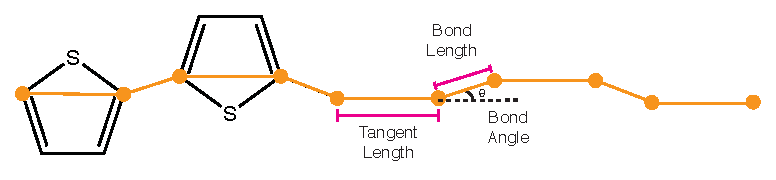
\includegraphics{figures/append_tor_model/course_grain_model.pdf}
    \caption{The course grained mapping for polythiophene. The tangent length, bond length, and bond angle are general inputs for the torsion potential model}
    \label{fig:cg_model}
\end{figure}

\begin{table}[hbt!]\centering
\caption{Torsion Potential Model Values}
\label{tab:tpm_vals}
\renewcommand{\arraystretch}{1.5}
\begin{threeparttable}
\begin{tabular}{cccc}\toprule
\multicolumn{1}{c}{\multirow{2}{3.5cm}{\centering }} &
\multicolumn{1}{c}{\multirow{2}{2.5cm}{\centering Tangent \\ Length (\AA)\tnote{\textdagger}}} &
\multicolumn{1}{c}{\multirow{2}{2.5cm}{\centering Bond \\ Length (\AA)\tnote{\textdagger}}} &
\multicolumn{1}{c}{\multirow{2}{2.5cm}{\centering Bond \\ Angle ($^\circ$)\tnote{*}}} \\ \\ \midrule
    Ground State & 2.47 & 1.46 & 15.2\\
    Doped State & 2.45 & 1.40 & 14.3\\
    Excited State & 2.50 & 1.35 & 14.1\\ \bottomrule
\end{tabular}
\begin{tablenotes}
\item[\textdagger] \footnotesize Taken from initial optimized geometry
\item[*] \footnotesize Boltzmann weighted average over all optimized torsion configurations
\end{tablenotes}
\end{threeparttable}
\end{table}

\subsection{Code}
The code used to generate chain conformations and collect chain statistics is freely available at \url{https://github.com/wood-b/dihedral_model}.

\section{Persistence Length \& End-to-end Distance}
\label{sec:lp}
\begin{equation}
\Large
\Big \langle \large \hat{\nu_i} \cdot \hat{\nu_j} \Big \rangle = \exp{\bigg(-\frac{N}{\chi l_{N}}\bigg)}
\label{eq:lN}
\end{equation}

\subsection{Tangent-tangent Correlation Function}

The tangent-tangent correlation function (eq. \ref{eq:lp}) can be rewritten into a form (SI eq. \ref{eq:lN}) that is easier to employ in practice by utilizing $L \approx m_lN$ and $l_p = m_ll_N$. The variable $l_N$ is the persistence length in monomer units ($N$). Additionally, the tangent-tangent correlation function can be normalized to decay from 1 by using unit backbone vectors ($\hat{\nu}$). Final $l_p$ values were computed by exponentially fitting the tangent-tangent correlation function \ref{eq:lN} and dimensionalizing $l_N$ using the relationship $l_p = m_ll_N$.

\subsection{Worm-like Chain Fitting}

End-to-end distances ($\sqrt{\big \langle R^2 \big \rangle}$) generated from the torsion potential model were compared with end-to-end distances from the 3D-WLC and the 2D-WLC (Figures \ref{fig:gs_wlc}, \ref{fig:d_wlc}, \ref{fig:e_wlc}). WLC end-to-end distances were calculated analytically using SI eq. \ref{eq:wlc_msqr}. Input $l_p$ values were computed from SI eq. \ref{eq:lN} using data from the torsion potential model and the appropriate $\chi$ value (i.e. $\chi = 1$ for 3D and $\chi = 2$ for 2D).

After comparing end-to-end distances of the WLC-3D, WLC-2D, and the torsion potential model it was clear that $l_p$ values for the torsion potential model could be improved by fitting $\chi$. $\chi$ values were determined by the ratio of the 3D-WLC $\big \langle R^2 \big \rangle$ and the torsion potential model $\big \langle R^2 \big \rangle$ at $N = 200$ for all values of $\alpha$ (Tables \ref{tab:d_lp} \ref{tab:e_lp}). In the end, $\chi$ values did not change that much over the range of $\alpha$ values. In the future, an average value of $\chi$ could be used.

\begin{equation}
\Large
\Big\langle R^2 \Big\rangle = 2l_p - 2l_p^2 \left(1 - e^{L/l_p} \right)
\label{eq:wlc_msqr}
\end{equation}

\begin{figure}[hbt!]
    \centering
    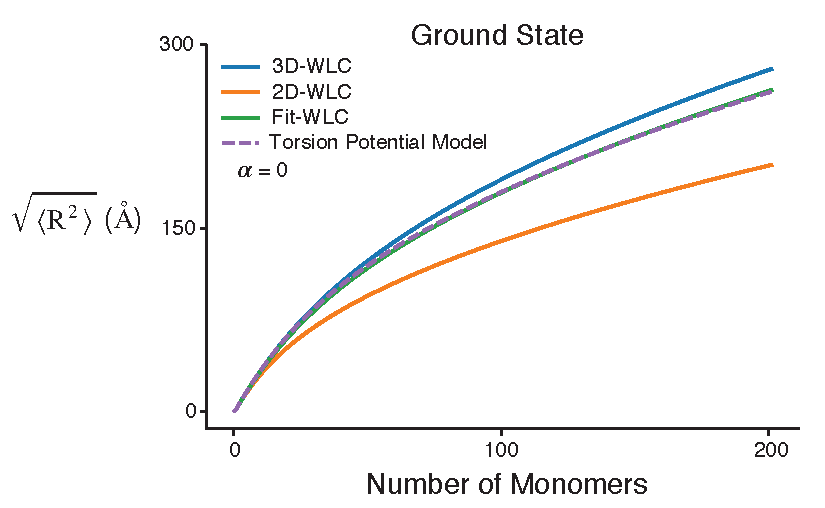
\includegraphics{figures/append_tor_model/gs_wlc_fit.pdf}
    \caption{Ground-state end-to-end distances for the 2D and 3D WLC, the torsion potential model, and the WLC where $\chi$ was fit to torsion potential model.}
    \label{fig:gs_wlc}
\end{figure}

\begin{figure}[hbt!]
    \centering
    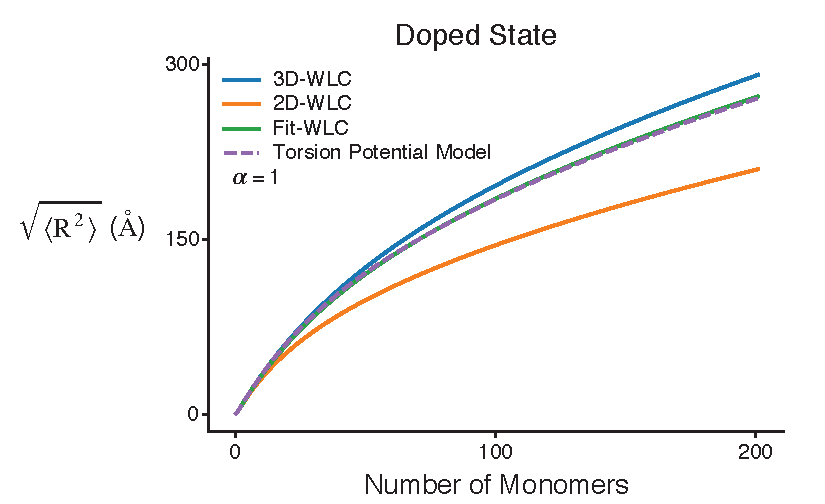
\includegraphics{figures/append_tor_model/cat_wlc_fit.pdf}
    \caption{Doped-state end-to-end distances for the 2D and 3D WLC, the torsion potential model, and the WLC where $\chi$ was fit to torsion potential model.}
    \label{fig:d_wlc}
\end{figure}

\begin{figure}[hbt!]
    \centering
    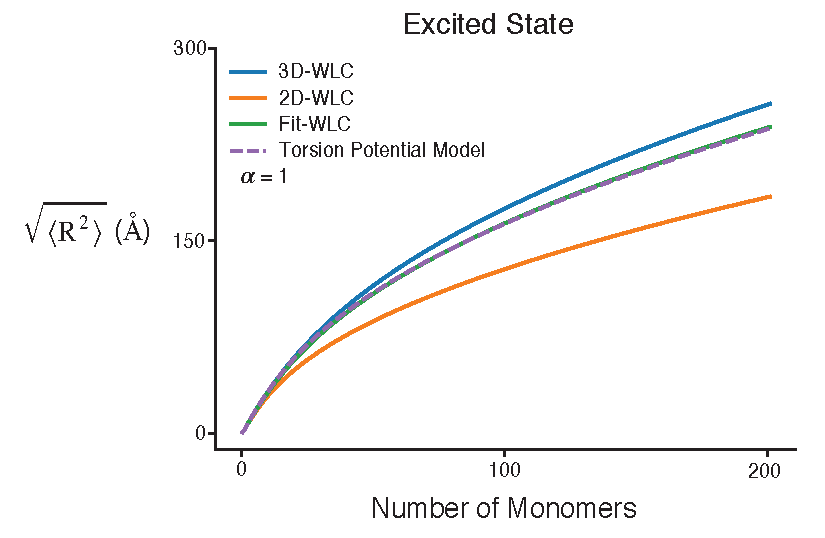
\includegraphics{figures/append_tor_model/trip_wlc_fit.pdf}
    \caption{Excited-state end-to-end distances for the 2D and 3D WLC, the torsion potential model, and the WLC where $\chi$ was fit to torsion potential model.}
    \label{fig:e_wlc}
\end{figure}

\clearpage
\subsection{Persistence Length Data}
\begin{table}[hbt!]\centering
\caption{Doped Persistence Length Values}
\label{tab:d_lp}
\renewcommand{\arraystretch}{1.5}
\begin{threeparttable}
\begin{tabular}{ccccc}\toprule
\multicolumn{1}{c}{\multirow{1}{3.5cm}{\centering $\alpha$}} &
\multicolumn{1}{c}{\multirow{1}{1.5cm}{\centering $\chi$}} &
\multicolumn{1}{c}{\multirow{1}{1.5cm}{\centering $m_l$}} &
\multicolumn{1}{c}{\multirow{1}{1.5cm}{\centering $l_p$}} & \\ \midrule
    0.0 & 1.147 & 3.88 & 4.74\\
    0.05 & 1.146 & 3.88 & 4.75\\
    0.1 & 1.151 & 3.87 & 4.77\\
    0.15 & 1.147 & 3.87 & 4.81\\
    0.2 & 1.146 & 3.87 & 4.84\\
    0.25 & 1.153 & 3.86 & 4.84\\
    0.3 & 1.147 & 3.86 & 4.88\\ \midrule
    0.35 & 1.148 & 3.86 & 4.91\\
    0.4 & 1.142 & 3.85 & 4.96\\
    0.45 & 1.156 & 3.85 & 4.90\\
    0.5 & 1.153 & 3.85 & 4.98\\
    0.55 & 1.146 & 3.84 & 5.03\\
    0.6 & 1.147 & 3.84 & 5.04\\
    0.65 & 1.149 & 3.83 & 5.08\\ \midrule
    0.7 & 1.149 & 3.83 & 5.10\\
    0.75 & 1.152 & 3.83 & 5.13\\
    0.8 & 1.151 & 3.82 & 5.15\\
    0.85 & 1.149 & 3.82 & 5.18\\
    0.9 & 1.151 & 3.82 & 5.20\\
    0.95 & 1.148 & 3.81 & 5.24\\
    1.0 & 1.154 & 3.81 & 5.22\\ \bottomrule
\end{tabular}
\begin{tablenotes}
\item
\end{tablenotes}
\end{threeparttable}
\end{table}

\begin{table}[hbt!]\centering
\caption{Excited Persistence Length Values}
\label{tab:e_lp}
\renewcommand{\arraystretch}{1.5}
\begin{threeparttable}
\begin{tabular}{ccccc}\toprule
\multicolumn{1}{c}{\multirow{1}{3.5cm}{\centering $\alpha$}} &
\multicolumn{1}{c}{\multirow{1}{1.5cm}{\centering $\chi$}} &
\multicolumn{1}{c}{\multirow{1}{1.5cm}{\centering $m_l$}} &
\multicolumn{1}{c}{\multirow{1}{1.5cm}{\centering $l_p$}} & \\ \midrule
    0.0 & 1.147 & 3.88 & 4.74\\
    0.05 & 1.146 & 3.88 & 4.70\\
    0.1 & 1.148 & 3.87 & 4.65\\
    0.15 & 1.146 & 3.87 & 4.61\\
    0.2 & 1.151 & 3.87 & 4.56\\
    0.25 & 1.152 & 3.86 & 4.52\\
    0.3 & 1.149 & 3.86 & 4.50\\ \midrule
    0.35 & 1.150 & 3.86 & 4.46\\
    0.4 & 1.150 & 3.85 & 4.42\\
    0.45 & 1.153 & 3.85 & 4.37\\
    0.5 & 1.155 & 3.85 & 4.32\\
    0.55 & 1.147 & 3.84 & 4.33\\
    0.6 & 1.154 & 3.84 & 4.27\\
    0.65 & 1.148 & 3.83 & 4.26\\ \midrule
    0.7 & 1.149 & 3.83 & 4.21\\
    0.75 & 1.152 & 3.83 & 4.16\\
    0.8 & 1.153 & 3.82 & 4.13\\
    0.85 & 1.154 & 3.82 & 4.09\\
    0.9 & 1.153 & 3.82 & 4.07\\
    0.95 & 1.151 & 3.81 & 4.03\\
    1.0 & 1.168 & 3.81 & 3.93\\ \bottomrule
\end{tabular}
\begin{tablenotes}
\item
\end{tablenotes}
\end{threeparttable}
\end{table}

\clearpage
\subsection{Sampled Torsion Angle Distributions}

Torsion angle histograms at different values of $\alpha$ (Figure \ref{fig:a_0_hist}, \ref{fig:a_025_hist}, \ref{fig:a_050_hist}, \ref{fig:a_075_hist}, and \ref{fig:a_1_hist}) demonstrate that excited chains consistently contained more cis (0\textdegree) \ torsion angles, which ultimately resulted in the excited chains being shorter.

\begin{figure}[hbt!]
    \centering
    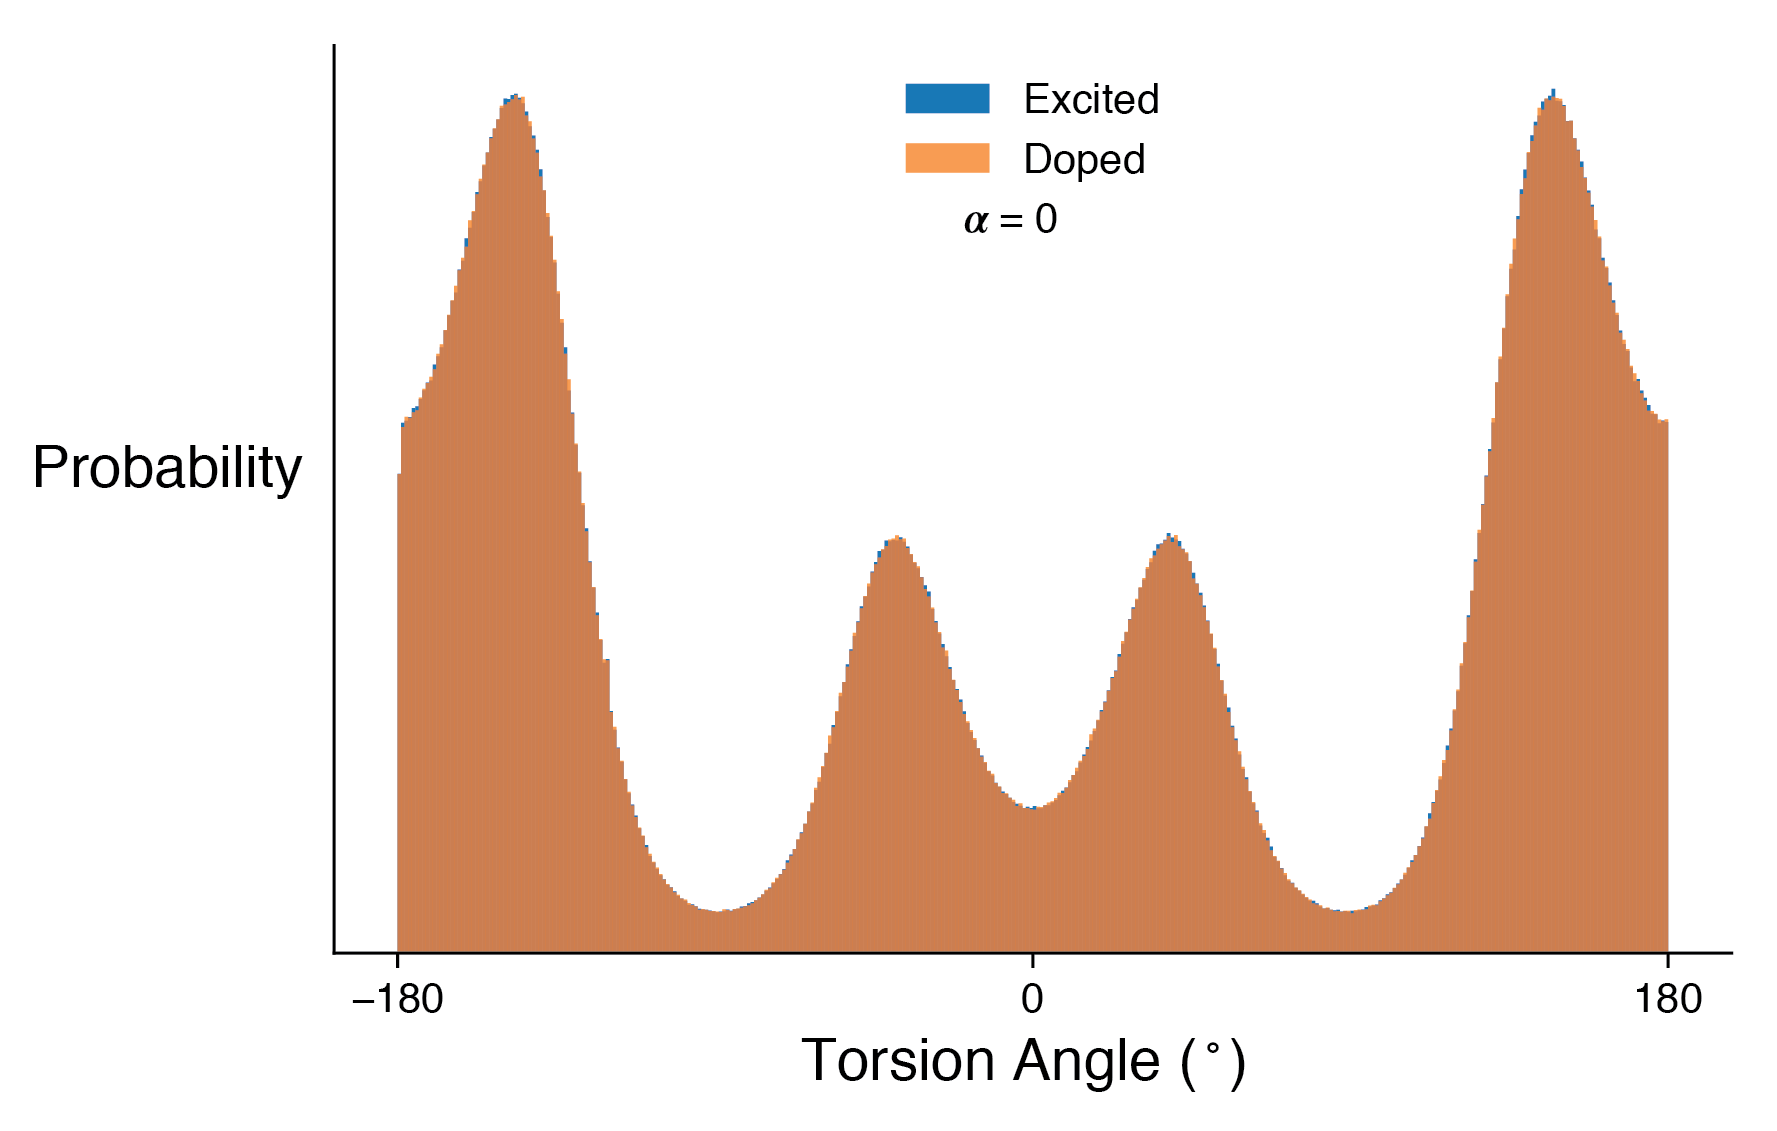
\includegraphics{figures/append_tor_model/a_0_hist.png}
    \caption{Overlaid histograms of doped and excited sampled torsion angles at $\alpha = 0$}
    \label{fig:a_0_hist}
\end{figure}

\begin{figure}[hbt!]
    \centering
    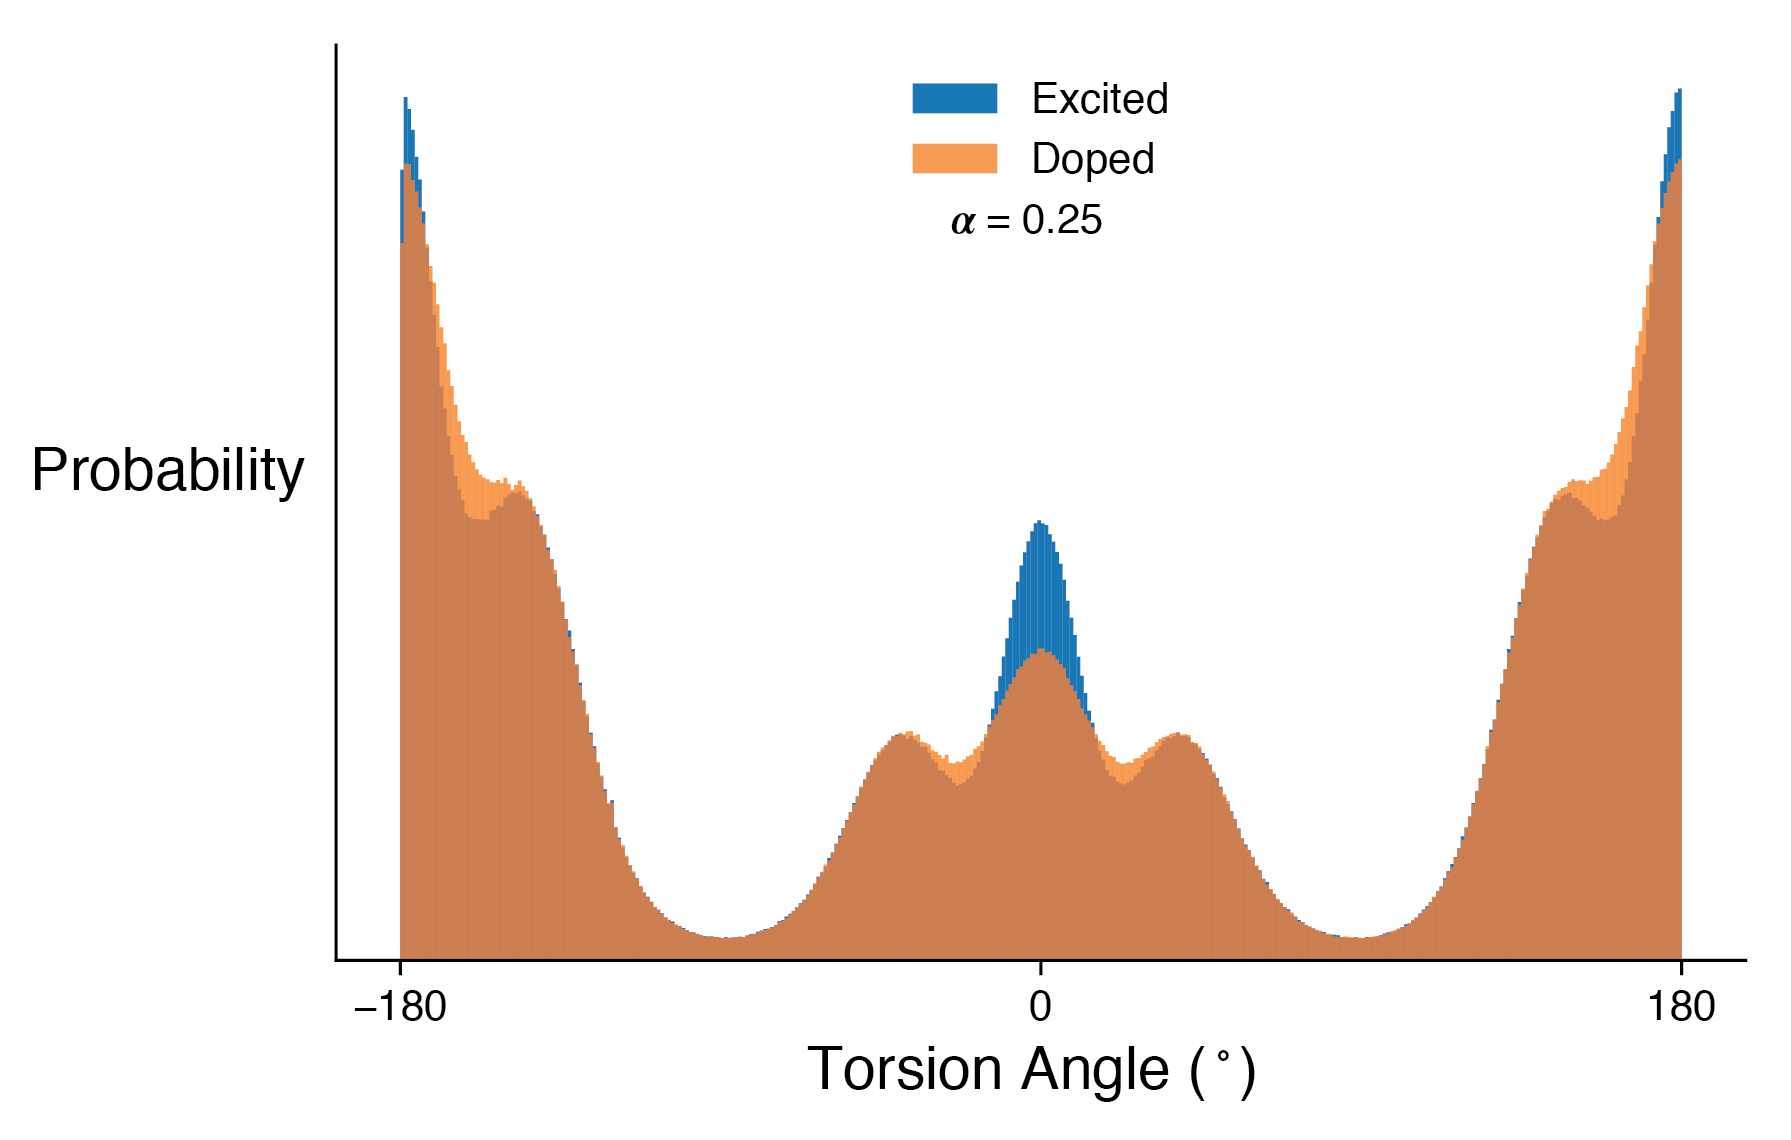
\includegraphics{figures/append_tor_model/a_025_hist.png}
    \caption{Overlaid histograms of doped and excited sampled torsion angles at $\alpha = 0.25$}
    \label{fig:a_025_hist}
\end{figure}

\begin{figure}[hbt!]
    \centering
    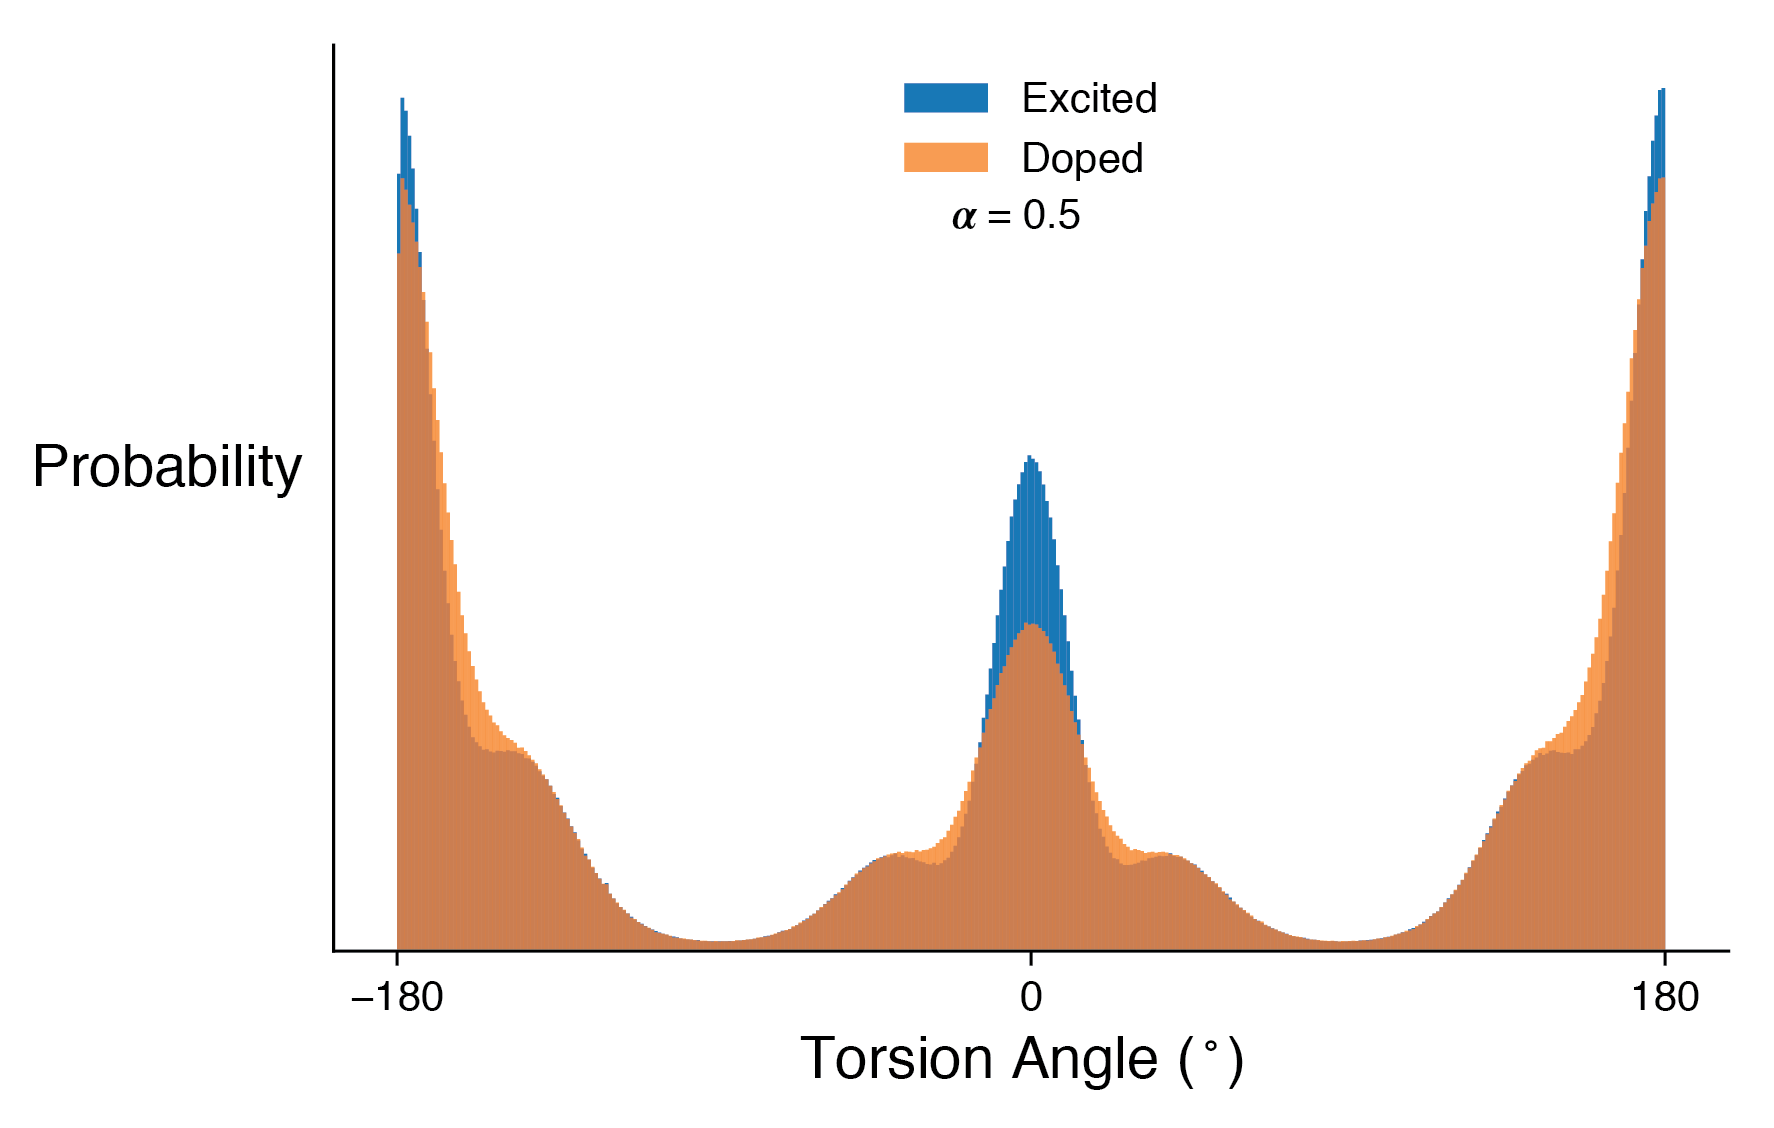
\includegraphics{figures/append_tor_model/a_050_hist.png}
    \caption{Overlaid histograms of doped and excited sampled torsion angles at $\alpha = 0.5$}
    \label{fig:a_050_hist}
\end{figure}

\begin{figure}[hbt!]
    \centering
    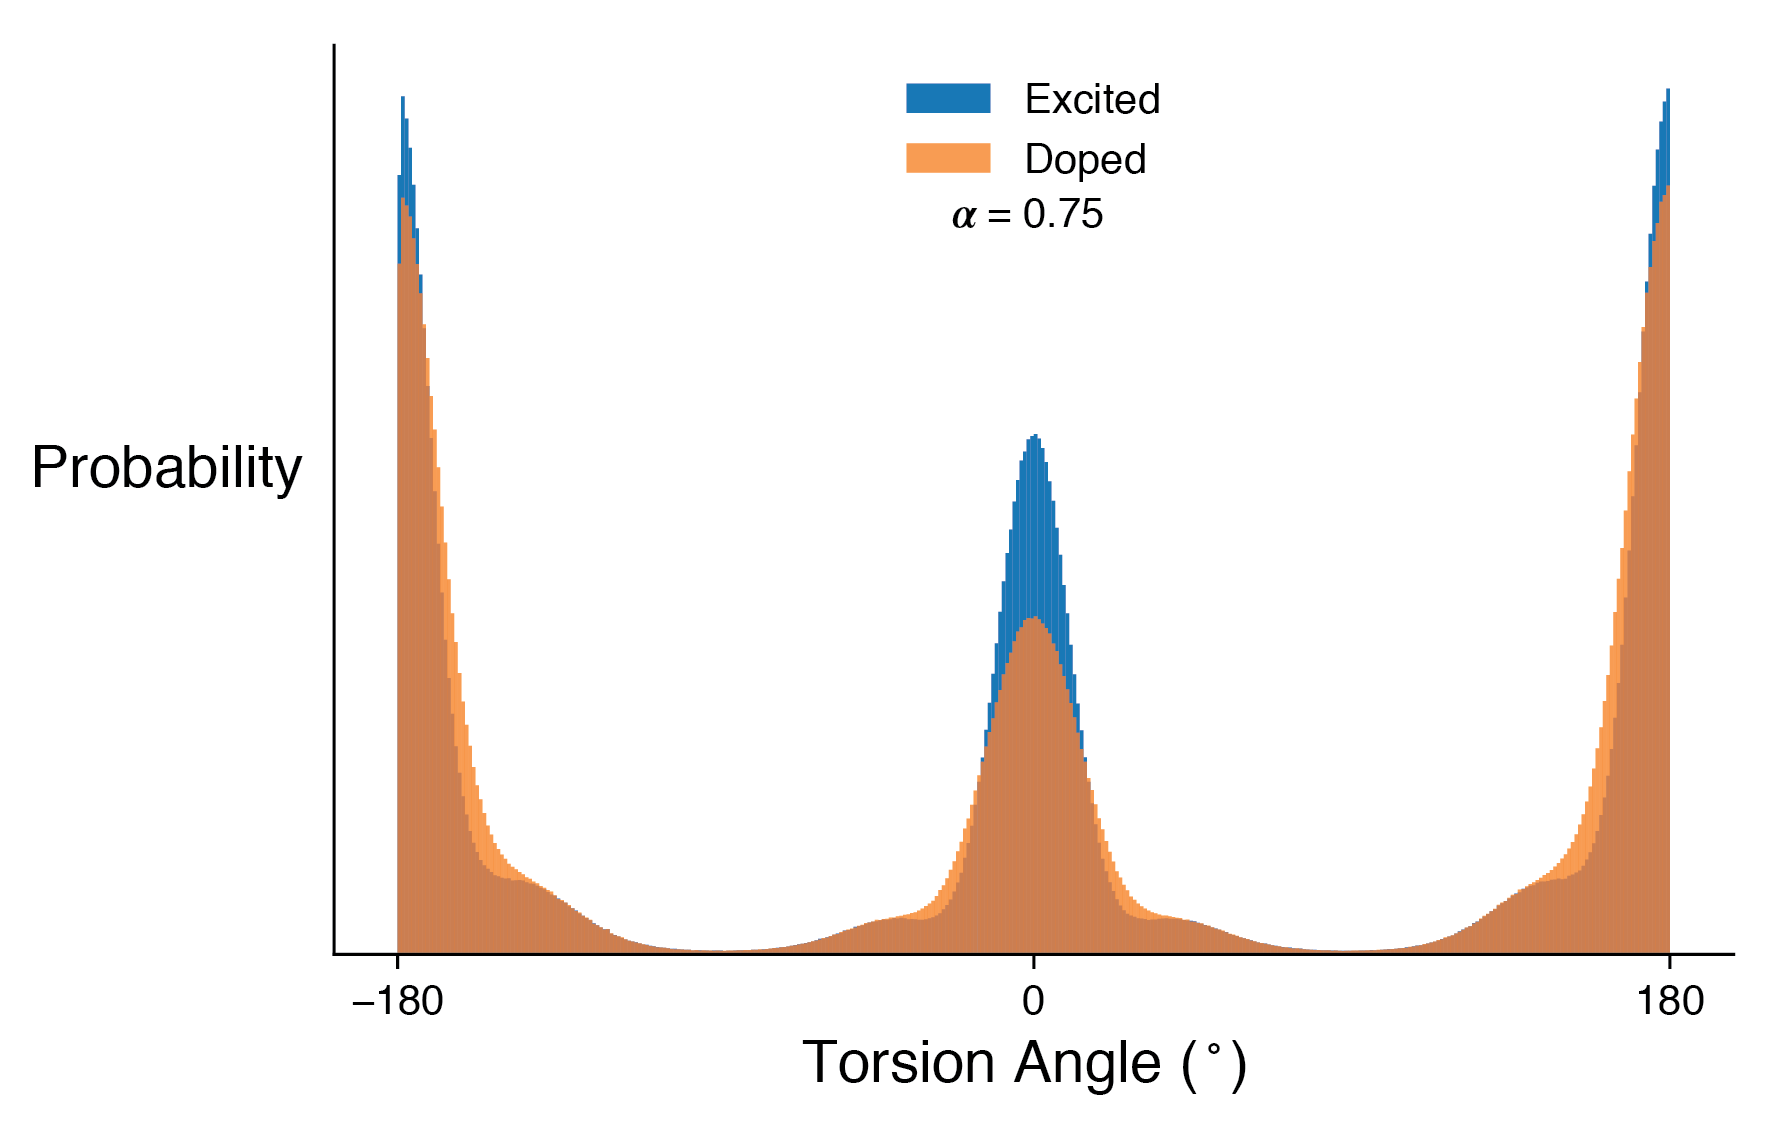
\includegraphics{figures/append_tor_model/a_075_hist.png}
    \caption{Overlaid histograms of doped and excited sampled torsion angles at $\alpha = 0.75$}
    \label{fig:a_075_hist}
\end{figure}

\begin{figure}[hbt!]
    \centering
    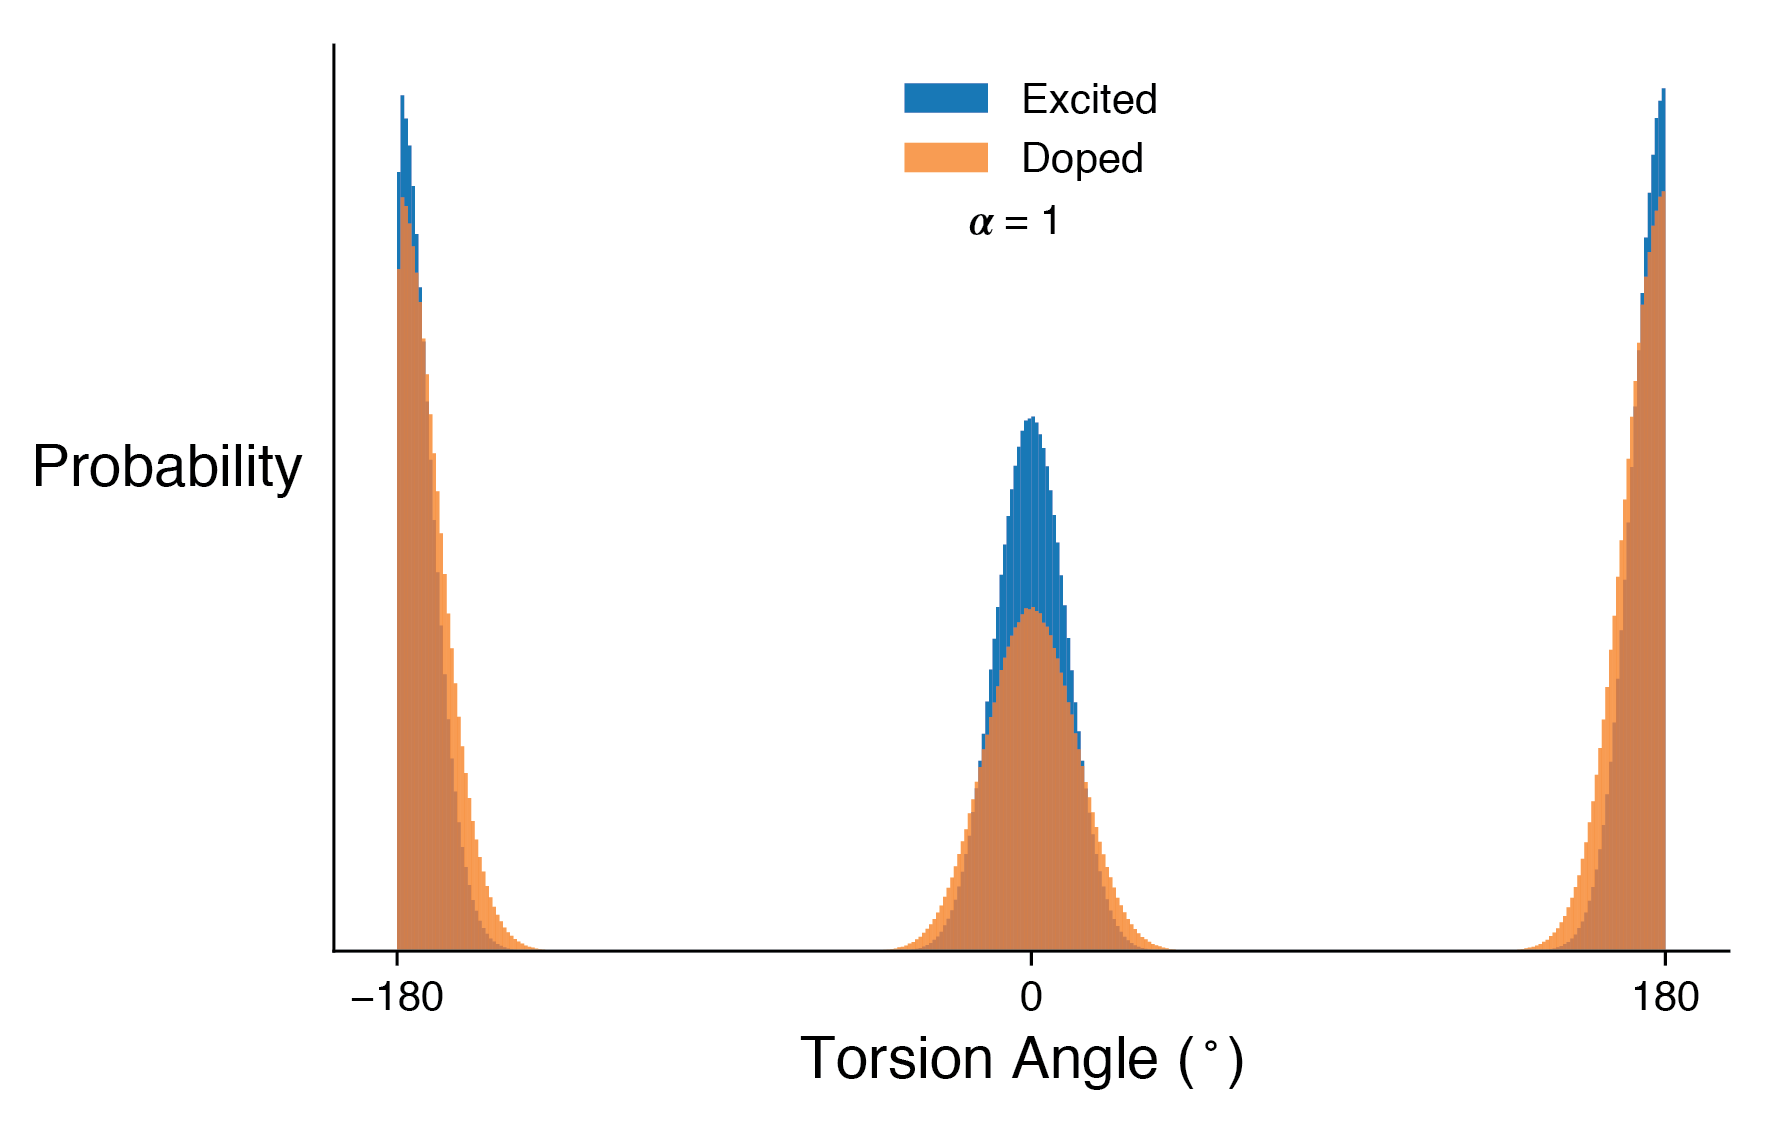
\includegraphics{figures/append_tor_model/a_1_hist.png}
    \caption{Overlaid histograms of doped and excited sampled torsion angles at $\alpha = 1$}
    \label{fig:a_1_hist}
\end{figure}

\clearpage
\section{Planarity}
\label{sec:planarity}
\subsection{Orientational Order Tensor}

The second rank orientational order tensor Q (SI eq. \ref{eq:Q}) was used to calculated the director and the S order parameter for each chain. The vectors used to describe chain planarity were the unit normal vectors ($\hat{e}$) to each thiophene ring along the chain (depicted in Figure \ref{fig:pt_vecs}). In SI eq. 1, $\hat{e} \otimes \hat{e}$ represents the outer product, which is equivalent to matrix multiplication of the column vector $\hat{e}$ and row vector $\hat{e}$. Additionally, $\mathds{1}$ represents the identity matrix. The parameter S and the director were determined by diagonalizing Q, where S is the largest eigenvalue and the director is the corresponding eigenvector.\cite{Allen2017}

\begin{equation}
\Large
\overleftrightarrow{Q} = \frac{1}{2N} \sum_{i=1}^{N} 3\hat{e_i} \otimes \hat{e_i} - \mathds{1}
\label{eq:Q}
\end{equation}
